\begin{frame}
	\frametitle{Vegetation}

	\begin{figure}
		\centering
		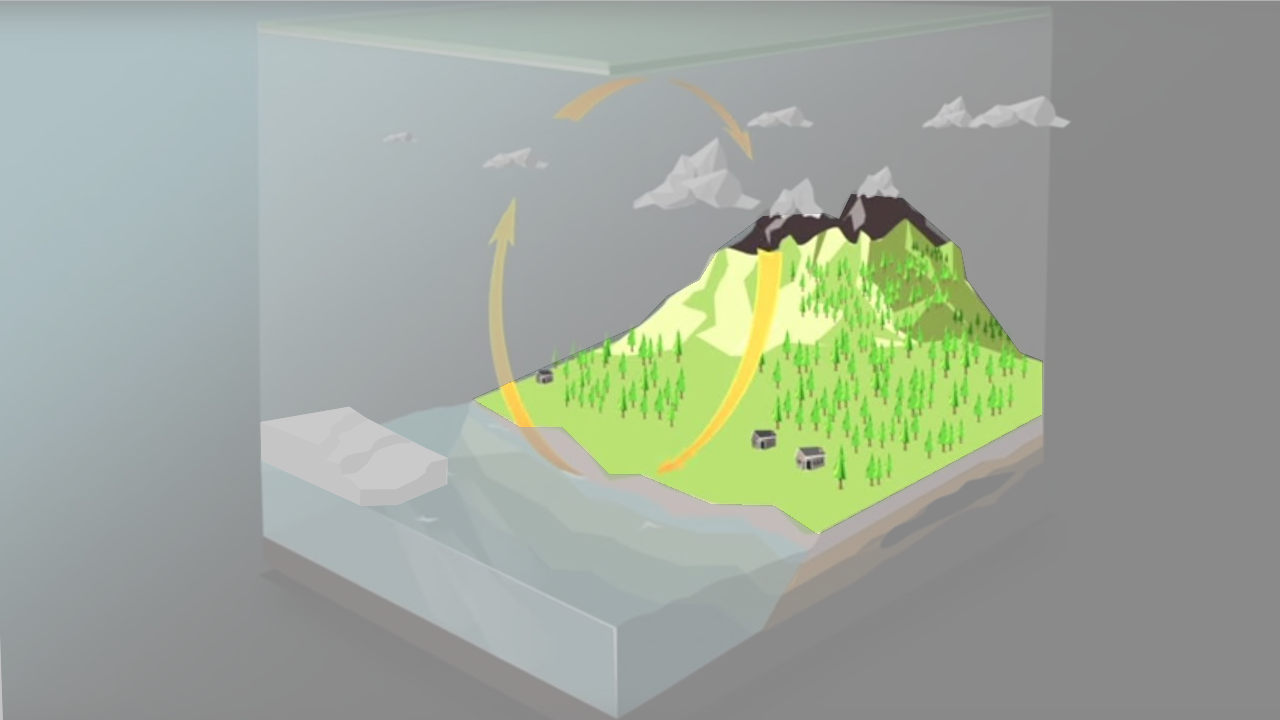
\includegraphics{bilder/WMO_Cycles_land.png}
		\caption{Die Vegetation ist eine interaktive Komponente des Klimasystems}
	\end{figure}

	\note{
		\begin{itemize}
			\item[] Vegetation ist sehr umfangreich und vielseitig
			\item[] steht in direktem Kontakt mit unterer Atmosphäre und Böden
			\item[] durch photosynthetische Prozesse und die Aufnahme sowie Abgabe von Wasser
			\item[] Vegetation hat dadurch massiven Einfluss auf Wetter und Klima - z.B. Tropischer Regenwald, Wolkenbildung
			\item[] zentral ist auch die Rolle beim Stoffkreislauf - u.a. Kohlenstoff, Phosphor, Nitrat, Stickstoff
			\item[] bietet Lebensraum und Lebensgrundlage
		\end{itemize}
	}
\end{frame}

\begin{frame}
	\frametitle{Vegetation}

  \begin{figure}
    \centering
    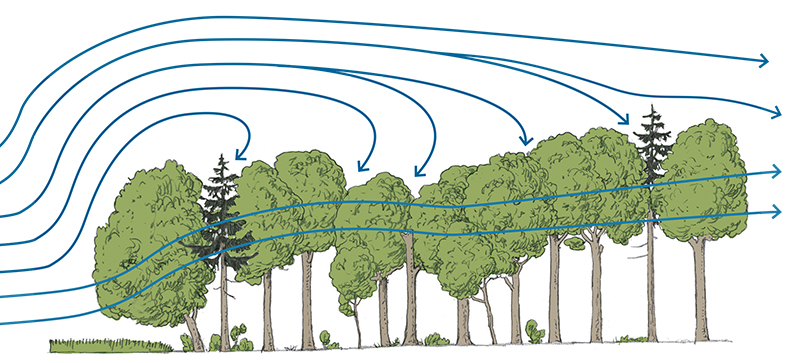
\includegraphics[width=.55\linewidth]{bilder/Wind_Vegetation.jpg}
    \caption{Wechselwirkung zwischen Atmosphäre und Biosphäre, Quelle: Stadt Kriens}
  \end{figure}
		\begin{itemize}
			\item Bodenbedeckung wirkt auf Wind, Wasseraustausch und Strahlungshaushalt
			\item [$\rightarrow$] Wälder bremsen Winde, speichern Wasser, beeinflussen Wolkenbildung und bilden Schatten und großen Lebensraum
			\item [$\rightarrow$] in Wüsten und Steppen versickert Wasser schneller und es gibt kaum Schatten, dafür existiert schwacher Albedo-Effekt
			\item Existenz und Wachstum von Vegetation bindet u.a. CO$_2$ und absorbiert Strahlung
			\item Absterben von Vegetation führt zu Freisetzung von CO$_2$ und anderen Stoffen in die Luft und Böden % Nitrat, Phosphat, Stickstoff etc.
		\end{itemize}

	\note{
		\begin{itemize}
			\item[] Photosynthese: Aufnahme von CO$_2$ und abgabe von O$_2$, Nutzung des Kohlenstoff für das Wachstum
			\item[] Lösung organischer Kohlenstoff-Verbindungen durch baterielle Zersetzung $\rightarrow$ Freisetzung von CO$_2$
		\end{itemize}
	}
\end{frame}
